% Options for packages loaded elsewhere
\PassOptionsToPackage{unicode}{hyperref}
\PassOptionsToPackage{hyphens}{url}
%
\documentclass[
]{article}
\usepackage{amsmath,amssymb}
\usepackage{lmodern}
\usepackage{ifxetex,ifluatex}
\ifnum 0\ifxetex 1\fi\ifluatex 1\fi=0 % if pdftex
  \usepackage[T1]{fontenc}
  \usepackage[utf8]{inputenc}
  \usepackage{textcomp} % provide euro and other symbols
\else % if luatex or xetex
  \usepackage{unicode-math}
  \defaultfontfeatures{Scale=MatchLowercase}
  \defaultfontfeatures[\rmfamily]{Ligatures=TeX,Scale=1}
\fi
% Use upquote if available, for straight quotes in verbatim environments
\IfFileExists{upquote.sty}{\usepackage{upquote}}{}
\IfFileExists{microtype.sty}{% use microtype if available
  \usepackage[]{microtype}
  \UseMicrotypeSet[protrusion]{basicmath} % disable protrusion for tt fonts
}{}
\makeatletter
\@ifundefined{KOMAClassName}{% if non-KOMA class
  \IfFileExists{parskip.sty}{%
    \usepackage{parskip}
  }{% else
    \setlength{\parindent}{0pt}
    \setlength{\parskip}{6pt plus 2pt minus 1pt}}
}{% if KOMA class
  \KOMAoptions{parskip=half}}
\makeatother
\usepackage{xcolor}
\IfFileExists{xurl.sty}{\usepackage{xurl}}{} % add URL line breaks if available
\IfFileExists{bookmark.sty}{\usepackage{bookmark}}{\usepackage{hyperref}}
\hypersetup{
  pdftitle={Part 2: Basic Inferential Data Analysis},
  pdfauthor={echf},
  hidelinks,
  pdfcreator={LaTeX via pandoc}}
\urlstyle{same} % disable monospaced font for URLs
\usepackage[margin=1in]{geometry}
\usepackage{color}
\usepackage{fancyvrb}
\newcommand{\VerbBar}{|}
\newcommand{\VERB}{\Verb[commandchars=\\\{\}]}
\DefineVerbatimEnvironment{Highlighting}{Verbatim}{commandchars=\\\{\}}
% Add ',fontsize=\small' for more characters per line
\usepackage{framed}
\definecolor{shadecolor}{RGB}{248,248,248}
\newenvironment{Shaded}{\begin{snugshade}}{\end{snugshade}}
\newcommand{\AlertTok}[1]{\textcolor[rgb]{0.94,0.16,0.16}{#1}}
\newcommand{\AnnotationTok}[1]{\textcolor[rgb]{0.56,0.35,0.01}{\textbf{\textit{#1}}}}
\newcommand{\AttributeTok}[1]{\textcolor[rgb]{0.77,0.63,0.00}{#1}}
\newcommand{\BaseNTok}[1]{\textcolor[rgb]{0.00,0.00,0.81}{#1}}
\newcommand{\BuiltInTok}[1]{#1}
\newcommand{\CharTok}[1]{\textcolor[rgb]{0.31,0.60,0.02}{#1}}
\newcommand{\CommentTok}[1]{\textcolor[rgb]{0.56,0.35,0.01}{\textit{#1}}}
\newcommand{\CommentVarTok}[1]{\textcolor[rgb]{0.56,0.35,0.01}{\textbf{\textit{#1}}}}
\newcommand{\ConstantTok}[1]{\textcolor[rgb]{0.00,0.00,0.00}{#1}}
\newcommand{\ControlFlowTok}[1]{\textcolor[rgb]{0.13,0.29,0.53}{\textbf{#1}}}
\newcommand{\DataTypeTok}[1]{\textcolor[rgb]{0.13,0.29,0.53}{#1}}
\newcommand{\DecValTok}[1]{\textcolor[rgb]{0.00,0.00,0.81}{#1}}
\newcommand{\DocumentationTok}[1]{\textcolor[rgb]{0.56,0.35,0.01}{\textbf{\textit{#1}}}}
\newcommand{\ErrorTok}[1]{\textcolor[rgb]{0.64,0.00,0.00}{\textbf{#1}}}
\newcommand{\ExtensionTok}[1]{#1}
\newcommand{\FloatTok}[1]{\textcolor[rgb]{0.00,0.00,0.81}{#1}}
\newcommand{\FunctionTok}[1]{\textcolor[rgb]{0.00,0.00,0.00}{#1}}
\newcommand{\ImportTok}[1]{#1}
\newcommand{\InformationTok}[1]{\textcolor[rgb]{0.56,0.35,0.01}{\textbf{\textit{#1}}}}
\newcommand{\KeywordTok}[1]{\textcolor[rgb]{0.13,0.29,0.53}{\textbf{#1}}}
\newcommand{\NormalTok}[1]{#1}
\newcommand{\OperatorTok}[1]{\textcolor[rgb]{0.81,0.36,0.00}{\textbf{#1}}}
\newcommand{\OtherTok}[1]{\textcolor[rgb]{0.56,0.35,0.01}{#1}}
\newcommand{\PreprocessorTok}[1]{\textcolor[rgb]{0.56,0.35,0.01}{\textit{#1}}}
\newcommand{\RegionMarkerTok}[1]{#1}
\newcommand{\SpecialCharTok}[1]{\textcolor[rgb]{0.00,0.00,0.00}{#1}}
\newcommand{\SpecialStringTok}[1]{\textcolor[rgb]{0.31,0.60,0.02}{#1}}
\newcommand{\StringTok}[1]{\textcolor[rgb]{0.31,0.60,0.02}{#1}}
\newcommand{\VariableTok}[1]{\textcolor[rgb]{0.00,0.00,0.00}{#1}}
\newcommand{\VerbatimStringTok}[1]{\textcolor[rgb]{0.31,0.60,0.02}{#1}}
\newcommand{\WarningTok}[1]{\textcolor[rgb]{0.56,0.35,0.01}{\textbf{\textit{#1}}}}
\usepackage{graphicx}
\makeatletter
\def\maxwidth{\ifdim\Gin@nat@width>\linewidth\linewidth\else\Gin@nat@width\fi}
\def\maxheight{\ifdim\Gin@nat@height>\textheight\textheight\else\Gin@nat@height\fi}
\makeatother
% Scale images if necessary, so that they will not overflow the page
% margins by default, and it is still possible to overwrite the defaults
% using explicit options in \includegraphics[width, height, ...]{}
\setkeys{Gin}{width=\maxwidth,height=\maxheight,keepaspectratio}
% Set default figure placement to htbp
\makeatletter
\def\fps@figure{htbp}
\makeatother
\setlength{\emergencystretch}{3em} % prevent overfull lines
\providecommand{\tightlist}{%
  \setlength{\itemsep}{0pt}\setlength{\parskip}{0pt}}
\setcounter{secnumdepth}{-\maxdimen} % remove section numbering
\ifluatex
  \usepackage{selnolig}  % disable illegal ligatures
\fi

\title{Part 2: Basic Inferential Data Analysis}
\author{echf}
\date{23/8/2021}

\begin{document}
\maketitle

\hypertarget{synopsis}{%
\subsection{Synopsis}\label{synopsis}}

\hypertarget{this-report-is-part-of-statistical-inference-course-from-johns-hopkins-university-coursera.}{%
\subparagraph{This report is part of Statistical Inference course from
Johns Hopkins University
(Coursera).}\label{this-report-is-part-of-statistical-inference-course-from-johns-hopkins-university-coursera.}}

\hypertarget{it-consists-of-two-parts}{%
\subsubsection{It consists of two
parts:}\label{it-consists-of-two-parts}}

\begin{enumerate}
\def\labelenumi{\arabic{enumi}.}
\tightlist
\item
  A simulation exercise.

  \begin{itemize}
  \tightlist
  \item
    will compare the exponential distribution in R with the Central
    Limit Theorem.
  \end{itemize}
\item
  Basic inferential data analysis.

  \begin{itemize}
  \tightlist
  \item
    I will analyze (very basically) the ToothGrowth data in the R
    datasets package.
  \end{itemize}
\end{enumerate}

\hypertarget{part-2-basic-inferential-data-analysis-with-toothgrowth-dataset}{%
\subsection{Part 2 : Basic inferential data analysis with ToothGrowth
dataset}\label{part-2-basic-inferential-data-analysis-with-toothgrowth-dataset}}

\hypertarget{toothgrowth-the-effect-of-vitamin-c-on-tooth-growth-in-guinea-pigs}{%
\paragraph{ToothGrowth: The Effect of Vitamin C on Tooth Growth in
Guinea
Pigs}\label{toothgrowth-the-effect-of-vitamin-c-on-tooth-growth-in-guinea-pigs}}

\hypertarget{description}{%
\subparagraph{Description}\label{description}}

\hypertarget{the-response-is-the-length-of-odontoblasts-cells-responsible-for-tooth-growth-in-60-guinea-pigs.-each-animal-received-one-of-three-dose}{%
\subparagraph{The response is the length of odontoblasts (cells
responsible for tooth growth) in 60 guinea pigs. Each animal received
one of three
dose}\label{the-response-is-the-length-of-odontoblasts-cells-responsible-for-tooth-growth-in-60-guinea-pigs.-each-animal-received-one-of-three-dose}}

levels of vitamin C (0.5, 1, and 2 mg/day) by one of two delivery
methods, orange juice or ascorbic acid (a form of vitamin C and coded as
VC).

\hypertarget{mission}{%
\paragraph{Mission}\label{mission}}

\begin{enumerate}
\def\labelenumi{\arabic{enumi}.}
\setcounter{enumi}{-1}
\tightlist
\item
  Load library's
\item
  Load the ToothGrowth data and perform some basic exploratory data
  analyses
\item
  Provide a basic summary of the data.
\item
  Use confidence intervals and/or hypothesis tests to compare tooth
  growth by Supplement and Dose.
\item
  State your conclusions and the assumptions needed for your
  conclusions.
\end{enumerate}

\hypertarget{load-librarys}{%
\subparagraph{Load library's}\label{load-librarys}}

\begin{Shaded}
\begin{Highlighting}[]
\NormalTok{echo }\OtherTok{=} \ConstantTok{TRUE}
\FunctionTok{options}\NormalTok{(}\AttributeTok{width=}\DecValTok{80}\NormalTok{)}
\FunctionTok{library}\NormalTok{(data.table)}
\FunctionTok{library}\NormalTok{(datasets)}
\FunctionTok{library}\NormalTok{(ggplot2)}
\end{Highlighting}
\end{Shaded}

\hypertarget{load-the-toothgrowth-data-and-perform-some-basic-exploratory-data-analyses}{%
\paragraph{Load the ToothGrowth data and perform some basic exploratory
data
analyses}\label{load-the-toothgrowth-data-and-perform-some-basic-exploratory-data-analyses}}

\begin{Shaded}
\begin{Highlighting}[]
\CommentTok{\# The Effect of Vitamin C on Tooth Growth in Guinea Pigs}
\FunctionTok{data}\NormalTok{(ToothGrowth)}
\NormalTok{toothGrowth }\OtherTok{\textless{}{-}} \FunctionTok{data.table}\NormalTok{(ToothGrowth) }
\FunctionTok{setnames}\NormalTok{(toothGrowth, }\FunctionTok{c}\NormalTok{(}\StringTok{\textquotesingle{}len\textquotesingle{}}\NormalTok{,}\StringTok{\textquotesingle{}supp\textquotesingle{}}\NormalTok{,}\StringTok{\textquotesingle{}dose\textquotesingle{}}\NormalTok{),}\FunctionTok{c}\NormalTok{(}\StringTok{\textquotesingle{}Length\textquotesingle{}}\NormalTok{,}\StringTok{\textquotesingle{}Supplement\textquotesingle{}}\NormalTok{,}\StringTok{\textquotesingle{}Dose\textquotesingle{}}\NormalTok{))}
\NormalTok{toothGrowth}\SpecialCharTok{$}\NormalTok{Dose }\OtherTok{\textless{}{-}} \FunctionTok{as.factor}\NormalTok{(toothGrowth}\SpecialCharTok{$}\NormalTok{Dose)}
\end{Highlighting}
\end{Shaded}

\hypertarget{as-we-see-there-are-60-observations-with-3-variables-in-this-data.-here-is-a-brief-explanation-of-the-variables-len-denotes-the-length-of-the-growth-supp-represents-the-delivery-supplement-type-either-vc-or-oj-and-dose-denotes-the-dose-in-milligramsday.-we-change-the-names-of-the-variables-to-length-supplement-and-dose-respectively.}{%
\subparagraph{As we see, there are 60 observations with 3 variables in
this data. Here is a brief explanation of the variables: len denotes the
length of the growth, supp represents the delivery (supplement) type
(either VC or OJ), and dose denotes the dose in milligrams/day. We
change the names of the variables to Length, Supplement, and Dose,
respectively.}\label{as-we-see-there-are-60-observations-with-3-variables-in-this-data.-here-is-a-brief-explanation-of-the-variables-len-denotes-the-length-of-the-growth-supp-represents-the-delivery-supplement-type-either-vc-or-oj-and-dose-denotes-the-dose-in-milligramsday.-we-change-the-names-of-the-variables-to-length-supplement-and-dose-respectively.}}

\hypertarget{basic-summary-of-the-data}{%
\subsubsection{Basic Summary of the
data}\label{basic-summary-of-the-data}}

\begin{Shaded}
\begin{Highlighting}[]
\FunctionTok{summary}\NormalTok{(toothGrowth)}
\end{Highlighting}
\end{Shaded}

\begin{verbatim}
##      Length      Supplement  Dose   
##  Min.   : 4.20   OJ:30      0.5:20  
##  1st Qu.:13.07   VC:30      1  :20  
##  Median :19.25              2  :20  
##  Mean   :18.81                      
##  3rd Qu.:25.27                      
##  Max.   :33.90
\end{verbatim}

\begin{Shaded}
\begin{Highlighting}[]
\FunctionTok{head}\NormalTok{(toothGrowth)}
\end{Highlighting}
\end{Shaded}

\begin{verbatim}
##    Length Supplement Dose
## 1:    4.2         VC  0.5
## 2:   11.5         VC  0.5
## 3:    7.3         VC  0.5
## 4:    5.8         VC  0.5
## 5:    6.4         VC  0.5
## 6:   10.0         VC  0.5
\end{verbatim}

\begin{Shaded}
\begin{Highlighting}[]
\NormalTok{ g}\OtherTok{\textless{}{-}}\FunctionTok{ggplot}\NormalTok{(toothGrowth, }\FunctionTok{aes}\NormalTok{(}\AttributeTok{x=}\NormalTok{Supplement, }\AttributeTok{y=}\NormalTok{Length, }\AttributeTok{color=}\NormalTok{Supplement)) }\SpecialCharTok{+}
    \FunctionTok{geom\_boxplot}\NormalTok{() }\SpecialCharTok{+} \FunctionTok{facet\_grid}\NormalTok{(}\AttributeTok{facets =} \SpecialCharTok{\textasciitilde{}}\NormalTok{ Dose) }\SpecialCharTok{+} 
   \FunctionTok{labs}\NormalTok{(}\AttributeTok{title=}\StringTok{"Tooth growth by supplement type and dose(mg)"}\NormalTok{ , }
        \AttributeTok{y =} \StringTok{"length"}\NormalTok{, }\AttributeTok{x =} \StringTok{"Supplement"}\NormalTok{)}
\NormalTok{ g}
\end{Highlighting}
\end{Shaded}

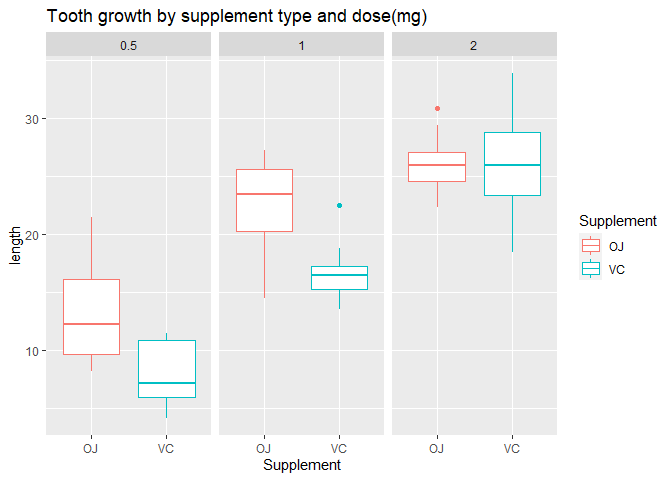
\includegraphics{Part-2--Basic-Inferential-Data-Analysis_files/figure-latex/unnamed-chunk-4-1.pdf}

\begin{Shaded}
\begin{Highlighting}[]
\CommentTok{\# Orange juice as delivery method of Vitamin C}
\NormalTok{oj }\OtherTok{\textless{}{-}} \FunctionTok{subset}\NormalTok{(ToothGrowth, supp }\SpecialCharTok{==} \StringTok{"OJ"}\NormalTok{)}
\CommentTok{\# Ascorbic acid as delivery method of Vitamin C}
\NormalTok{vc }\OtherTok{\textless{}{-}} \FunctionTok{subset}\NormalTok{(ToothGrowth, supp }\SpecialCharTok{==} \StringTok{"VC"}\NormalTok{)}
\end{Highlighting}
\end{Shaded}

\hypertarget{we-want-to-see-if-delivering-vitamin-c-via-orange-juice-enhances-more-tooth-growth-in-guinea-pigs-than-ascorbic-acid.-a-one-sided-hypothesis-test-will-be-conducted.-since-we-are-not-told-whether-the-variances-are-equal-or-not-we-will-assume-unequal-variances-to-be-on-the-conservative-side.-we-will-use-the-default-95-confidence-level.}{%
\subparagraph{We want to see if delivering vitamin C via orange juice
enhances more tooth growth in guinea pigs than ascorbic acid. A
one-sided hypothesis test will be conducted. Since we are not told
whether the variances are equal or not, we will assume unequal variances
to be on the conservative side. We will use the default, 95\% confidence
level.}\label{we-want-to-see-if-delivering-vitamin-c-via-orange-juice-enhances-more-tooth-growth-in-guinea-pigs-than-ascorbic-acid.-a-one-sided-hypothesis-test-will-be-conducted.-since-we-are-not-told-whether-the-variances-are-equal-or-not-we-will-assume-unequal-variances-to-be-on-the-conservative-side.-we-will-use-the-default-95-confidence-level.}}

\begin{Shaded}
\begin{Highlighting}[]
\FunctionTok{t.test}\NormalTok{(oj}\SpecialCharTok{$}\NormalTok{len, vc}\SpecialCharTok{$}\NormalTok{len, }\AttributeTok{alternative =} \StringTok{"greater"}\NormalTok{, }\AttributeTok{var.equal =} \ConstantTok{FALSE}\NormalTok{)}
\end{Highlighting}
\end{Shaded}

\begin{verbatim}
## 
##  Welch Two Sample t-test
## 
## data:  oj$len and vc$len
## t = 1.9153, df = 55.309, p-value = 0.03032
## alternative hypothesis: true difference in means is greater than 0
## 95 percent confidence interval:
##  0.4682687       Inf
## sample estimates:
## mean of x mean of y 
##  20.66333  16.96333
\end{verbatim}

\hypertarget{the-result-shows-a-t-statistic-of-1.9153-with-55.3-degrees-of-freedom.-the-p-value-is-0.03.-the-95-confidence-interval-is-0.47-inf.-from-the-result-delivery-using-orange-juice-seems-to-be-statistically-better-than-delivery-via-ascorbic-acid-for-tooth-growth-in-guinea-pigs.}{%
\subparagraph{The result shows a t-statistic of 1.9153 with 55.3 degrees
of freedom. The P-value is 0.03. The 95\% confidence interval is (0.47,
inf). From the result, delivery using orange juice seems to be
statistically better than delivery via ascorbic acid for tooth growth in
guinea
pigs.}\label{the-result-shows-a-t-statistic-of-1.9153-with-55.3-degrees-of-freedom.-the-p-value-is-0.03.-the-95-confidence-interval-is-0.47-inf.-from-the-result-delivery-using-orange-juice-seems-to-be-statistically-better-than-delivery-via-ascorbic-acid-for-tooth-growth-in-guinea-pigs.}}

\hypertarget{if-you-switch-variables-use-alternative-less.}{%
\subparagraph{If you switch variables, use alternative =
``less''.}\label{if-you-switch-variables-use-alternative-less.}}

\begin{Shaded}
\begin{Highlighting}[]
\FunctionTok{t.test}\NormalTok{(vc}\SpecialCharTok{$}\NormalTok{len, oj}\SpecialCharTok{$}\NormalTok{len, }\AttributeTok{alternative =} \StringTok{"less"}\NormalTok{, }\AttributeTok{var.equal =} \ConstantTok{FALSE}\NormalTok{)}
\end{Highlighting}
\end{Shaded}

\begin{verbatim}
## 
##  Welch Two Sample t-test
## 
## data:  vc$len and oj$len
## t = -1.9153, df = 55.309, p-value = 0.03032
## alternative hypothesis: true difference in means is less than 0
## 95 percent confidence interval:
##        -Inf -0.4682687
## sample estimates:
## mean of x mean of y 
##  16.96333  20.66333
\end{verbatim}

\hypertarget{both-one-sided-hypothesis-show-the-same-p-value-and-degrees-of-freedom.-the-t-statistic-is-negative-of-the-other-and-the-confidence-interval-goes-in-the-other-direction.}{%
\subparagraph{Both one-sided hypothesis show the same P-value and
degrees of freedom. The t-statistic is negative of the other and the
confidence interval goes in the other
direction.}\label{both-one-sided-hypothesis-show-the-same-p-value-and-degrees-of-freedom.-the-t-statistic-is-negative-of-the-other-and-the-confidence-interval-goes-in-the-other-direction.}}

\hypertarget{comparisons-of-dose}{%
\paragraph{Comparisons of dose}\label{comparisons-of-dose}}

\hypertarget{comparison-of-dose-0.5-and-1-0.5-vs-2-and-1-vs-2-with-t.-test-i-assume-data-are-normally-distributed}{%
\subparagraph{Comparison of dose 0.5 and 1, 0.5 vs 2, and 1 vs 2 with t.
test (I assume data are normally
distributed)}\label{comparison-of-dose-0.5-and-1-0.5-vs-2-and-1-vs-2-with-t.-test-i-assume-data-are-normally-distributed}}

\begin{Shaded}
\begin{Highlighting}[]
\NormalTok{dose5}\OtherTok{\textless{}{-}}\FunctionTok{subset}\NormalTok{(ToothGrowth, ToothGrowth}\SpecialCharTok{$}\NormalTok{dose }\SpecialCharTok{==} \FloatTok{0.5}\NormalTok{)}
\NormalTok{dose1}\OtherTok{\textless{}{-}}\FunctionTok{subset}\NormalTok{(ToothGrowth, ToothGrowth}\SpecialCharTok{$}\NormalTok{dose }\SpecialCharTok{==} \DecValTok{1}\NormalTok{)}
\NormalTok{dose2}\OtherTok{\textless{}{-}}\FunctionTok{subset}\NormalTok{(ToothGrowth, ToothGrowth}\SpecialCharTok{$}\NormalTok{dose }\SpecialCharTok{==} \DecValTok{2}\NormalTok{)}
\end{Highlighting}
\end{Shaded}

\begin{Shaded}
\begin{Highlighting}[]
\DocumentationTok{\#\#\#\#\# dose 0.5 vs 1}
\FunctionTok{t.test}\NormalTok{(dose5}\SpecialCharTok{$}\NormalTok{len,dose1}\SpecialCharTok{$}\NormalTok{len, }\AttributeTok{var.equal =}\NormalTok{ T, }\AttributeTok{paired =}\NormalTok{ F)}
\end{Highlighting}
\end{Shaded}

\begin{verbatim}
## 
##  Two Sample t-test
## 
## data:  dose5$len and dose1$len
## t = -6.4766, df = 38, p-value = 1.266e-07
## alternative hypothesis: true difference in means is not equal to 0
## 95 percent confidence interval:
##  -11.983748  -6.276252
## sample estimates:
## mean of x mean of y 
##    10.605    19.735
\end{verbatim}

\begin{Shaded}
\begin{Highlighting}[]
\DocumentationTok{\#\#\#\#\# dose 0.5 vs 2 }
\FunctionTok{t.test}\NormalTok{(dose5}\SpecialCharTok{$}\NormalTok{len,dose2}\SpecialCharTok{$}\NormalTok{len, }\AttributeTok{var.equal =}\NormalTok{ F, }\AttributeTok{paired =}\NormalTok{ F)}
\end{Highlighting}
\end{Shaded}

\begin{verbatim}
## 
##  Welch Two Sample t-test
## 
## data:  dose5$len and dose2$len
## t = -11.799, df = 36.883, p-value = 4.398e-14
## alternative hypothesis: true difference in means is not equal to 0
## 95 percent confidence interval:
##  -18.15617 -12.83383
## sample estimates:
## mean of x mean of y 
##    10.605    26.100
\end{verbatim}

\begin{Shaded}
\begin{Highlighting}[]
\DocumentationTok{\#\#\#\#\#  dose 1 vs 2" }
\FunctionTok{t.test}\NormalTok{(dose1}\SpecialCharTok{$}\NormalTok{len,dose2}\SpecialCharTok{$}\NormalTok{len, }\AttributeTok{var.equal =}\NormalTok{ F, }\AttributeTok{paired =}\NormalTok{ F)}
\end{Highlighting}
\end{Shaded}

\begin{verbatim}
## 
##  Welch Two Sample t-test
## 
## data:  dose1$len and dose2$len
## t = -4.9005, df = 37.101, p-value = 1.906e-05
## alternative hypothesis: true difference in means is not equal to 0
## 95 percent confidence interval:
##  -8.996481 -3.733519
## sample estimates:
## mean of x mean of y 
##    19.735    26.100
\end{verbatim}

\hypertarget{here-we-can-see-that-the-null-hypothesis-has-been-rejected-for-all-dose-comparisons.-therefore-we-can-conclude-that-dose-without-regarding-supplementation-has-an-effect-on-teeth-growth.}{%
\subparagraph{Here we can see that the null hypothesis has been rejected
for all dose comparisons. Therefore we can conclude that dose, without
regarding supplementation, has an effect on teeth
growth.}\label{here-we-can-see-that-the-null-hypothesis-has-been-rejected-for-all-dose-comparisons.-therefore-we-can-conclude-that-dose-without-regarding-supplementation-has-an-effect-on-teeth-growth.}}

\hypertarget{calculating-confidence-interval}{%
\paragraph{Calculating Confidence
Interval}\label{calculating-confidence-interval}}

\hypertarget{to-calculate-the-confidence-interval-only-append-conf.int-after-the-t.test-function.-there-is-no-need-to-enter-mu-as-mu-is-not-part-of-the-confidence-interval-computation.-if-no-confidence-level-is-specified-r-defaults-to-95.}{%
\subparagraph{To calculate the confidence interval only, append
\$conf.int after the t.test( ) function. There is no need to enter mu as
mu is not part of the confidence interval computation. If no confidence
level is specified, R defaults to
95\%.}\label{to-calculate-the-confidence-interval-only-append-conf.int-after-the-t.test-function.-there-is-no-need-to-enter-mu-as-mu-is-not-part-of-the-confidence-interval-computation.-if-no-confidence-level-is-specified-r-defaults-to-95.}}

\begin{Shaded}
\begin{Highlighting}[]
\CommentTok{\# Vitamin C delivery via orange juice at 2 ml/day}
\NormalTok{oj\_two }\OtherTok{\textless{}{-}} \FunctionTok{subset}\NormalTok{(ToothGrowth, ToothGrowth}\SpecialCharTok{$}\NormalTok{supp }\SpecialCharTok{==} \StringTok{"OJ"} \SpecialCharTok{\&}\NormalTok{ ToothGrowth}\SpecialCharTok{$}\NormalTok{dose }\SpecialCharTok{==} \StringTok{"2"}\NormalTok{)}
\end{Highlighting}
\end{Shaded}

\begin{Shaded}
\begin{Highlighting}[]
\CommentTok{\# Vitamin C delivery via ascorbic acid at 2 ml/day}
\NormalTok{vc\_two }\OtherTok{\textless{}{-}} \FunctionTok{subset}\NormalTok{(ToothGrowth, ToothGrowth}\SpecialCharTok{$}\NormalTok{supp }\SpecialCharTok{==} \StringTok{"VC"} \SpecialCharTok{\&}\NormalTok{ ToothGrowth}\SpecialCharTok{$}\NormalTok{dose }\SpecialCharTok{==} \StringTok{"2"}\NormalTok{)}
\end{Highlighting}
\end{Shaded}

\begin{Shaded}
\begin{Highlighting}[]
\CommentTok{\# Default is 95\% confidence level}
\FunctionTok{t.test}\NormalTok{(oj\_two}\SpecialCharTok{$}\NormalTok{len, vc\_two}\SpecialCharTok{$}\NormalTok{len, }\AttributeTok{var.equal =} \ConstantTok{FALSE}\NormalTok{)}\SpecialCharTok{$}\NormalTok{conf.int}
\end{Highlighting}
\end{Shaded}

\begin{verbatim}
## [1] -3.79807  3.63807
## attr(,"conf.level")
## [1] 0.95
\end{verbatim}

\begin{Shaded}
\begin{Highlighting}[]
\CommentTok{\# To calculate 99\% confidence level}
\FunctionTok{t.test}\NormalTok{(oj\_two}\SpecialCharTok{$}\NormalTok{len, vc\_two}\SpecialCharTok{$}\NormalTok{len, }\AttributeTok{var.equal =} \ConstantTok{FALSE}\NormalTok{, }\AttributeTok{conf.level =} \FloatTok{0.99}\NormalTok{)}\SpecialCharTok{$}\NormalTok{conf.int}
\end{Highlighting}
\end{Shaded}

\begin{verbatim}
## [1] -5.239603  5.079603
## attr(,"conf.level")
## [1] 0.99
\end{verbatim}

\hypertarget{conclusions}{%
\paragraph{Conclusions}\label{conclusions}}

\hypertarget{the-conclusion-is-when-the-dose-is-0.5-or-1.0-there-is-a-difference-between-the-teeth-growth-after-taking-oj-and-vc-while-when-the-dose-is-2.0-there-is-no-difference-between-the-teeth-growth-after-taking-oj-and-vc.-the-assumption-needed-is-we-first-assumed-the-whole-population-is-normally-distributed-then-we-assumed-the-population-is-normally-distributed-under-each-dose.}{%
\subparagraph{The conclusion is when the dose is 0.5 or 1.0 there is a
difference between the teeth growth after taking OJ and VC, while when
the dose is 2.0, there is no difference between the teeth growth after
taking OJ and VC. The assumption needed is we first assumed the whole
population is normally distributed, then we assumed the population is
normally distributed under each
dose.}\label{the-conclusion-is-when-the-dose-is-0.5-or-1.0-there-is-a-difference-between-the-teeth-growth-after-taking-oj-and-vc-while-when-the-dose-is-2.0-there-is-no-difference-between-the-teeth-growth-after-taking-oj-and-vc.-the-assumption-needed-is-we-first-assumed-the-whole-population-is-normally-distributed-then-we-assumed-the-population-is-normally-distributed-under-each-dose.}}

\hypertarget{section}{%
\subparagraph{--------}\label{section}}

\end{document}
